\documentclass[fleqn,t,serif,10pt,aspectratio=141,compress]{beamer}
\usepackage{preamble}
\usepackage{bm}

\begin{document}
{
\setbeamercolor{background canvas}{bg=OPBlue}
\begin{frame}[c,plain]
    \vspace{8pt}
    \begin{tcolorbox}[colframe=cyan]
        \begin{tcolorbox}[colback=OPBlue,colframe=black,colupper=white,]
            \centering
            {\Large \textbf{
            Hamiltonian Topological Optics
            }}

            \medskip
            \textbf{Dr. M. Perry Nerem}
        \end{tcolorbox}
        
        \centering
        \medskip
        SPS -- Speed Researching        

        \medskip
        \begin{tcolorbox}[
            enhanced, clip upper,
            colframe=black,
            boxsep=0pt,
            left=0pt,
            right=0pt,
            top=2pt,
            bottom=0pt,
            width=.6\textwidth,
        ]
            \centering
            \movie[autostart,loop]{\includegraphics[width=\textwidth]{initial-conditions-0.png}}
                {initial-conditions.gif}    
        \end{tcolorbox}

        \today
    \end{tcolorbox}
\end{frame}
}

\begin{frame}{Topological Physics}
    Q: What does topology mean for an optical system?
    \begin{itemize}
        \item 
            \red{Topology} is the study of materials and what happens to their
            physical properties under deformations.
        \item A topological insulator (TI) exploits the electrical properties in atom configuration.
            \begin{center}
                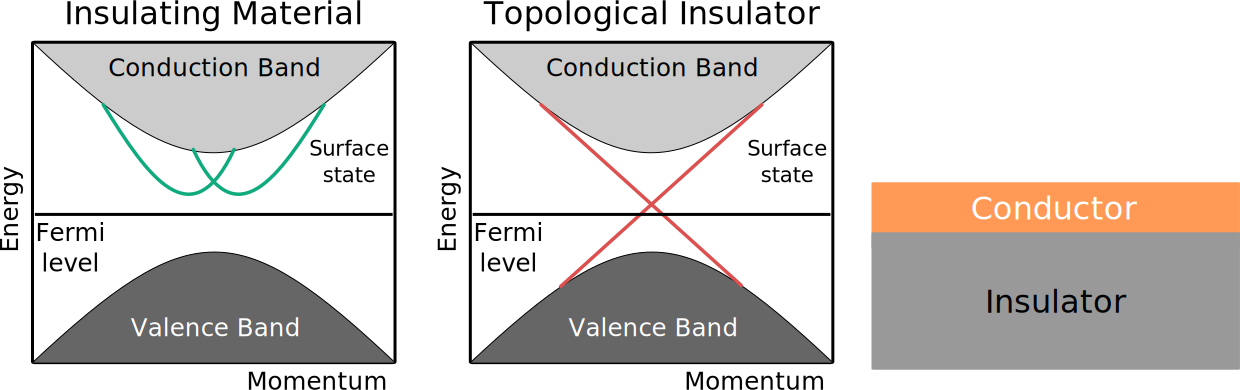
\includegraphics[width=.75\textwidth]{TI-figur.pdf}
            \end{center}
        \item Simple model of a TI: two sheets of electrons with anti-parallel magnetic fields.
            \begin{center}
                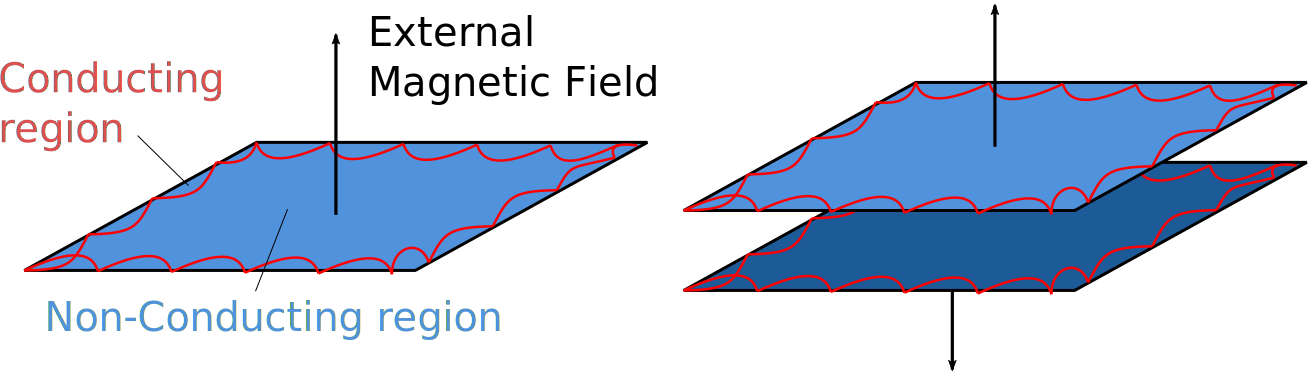
\includegraphics[width=.75\textwidth]{TI-electron-sheet-model.pdf}
            \end{center}
    \end{itemize}
\end{frame}

\begin{frame}{Topological Optics}
    Design new techniques to control the phase or \textit{trajectories} of rays.

    \begin{columns}
        \begin{column}{.40\textwidth}
            ~\\
            \vspace{1cm}
            \includegraphics[width=\textwidth]{Light-Pipe-Concept.pdf}
        \end{column}
        \begin{column}{.65\textwidth}
            ~\\
            \movie{\includegraphics[width=\textwidth]{targer-001.png}}
                  {optical-topological-change.mp4}
        \end{column}
    \end{columns}
\end{frame}

\begin{frame}{Prerequisites to start this research}
    \begin{itemize}
        \item \textbf{If you can numerically integrate $\bm{\dot{x}=F(t,x)}$ you can start right now!}
        \item \textbf{Hamiltonian Mechanics}
            \begin{equation*}
                H(q,p)=\frac{p^2}{2m}+V(q)
                \quad \Rightarrow \quad
                \dot{q}=\frac{\partial H}{\partial p}, \quad
                \dot{p}=-\frac{\partial H}{\partial q}
            \end{equation*}
        \item \textbf{Hamilton's Optomechanical Analogy}

            Fermat's Principle of Least Time: Light path minimizing time \\
            Maupertuis' Principle of Least Action: Classical path minimizing action
            \begin{center}
                \includegraphics[width=.7\textwidth]{Opto-Mechanical-Analogy.pdf}

                \begin{tcolorbox}[
                colframe=cyan,
                ]
                    \centering
                    Simulate \blue{optical} paths using \red{classical} trajectories.
                \end{tcolorbox}
            \end{center}
    \end{itemize}
\end{frame}
\end{document}
